%% This template can be used to write a paper for
%% Computer Physics Communications using LaTeX.
%% For authors who want to write a computer program description,
%% an example Program Summary is included that only has to be
%% completed and which will give the correct layout in the
%% preprint and the journal.
%% The `elsarticle' style is used and more information on this style
%% can be found at 
%% http://www.elsevier.com/wps/find/authorsview.authors/elsarticle.
%%
%%
\documentclass[preprint,12pt]{elsarticle}

%% Use the option review to obtain double line spacing
%% \documentclass[preprint,review,12pt]{elsarticle}

%% Use the options 1p,twocolumn; 3p; 3p,twocolumn; 5p; or 5p,twocolumn
%% for a journal layout:
%% \documentclass[final,1p,times]{elsarticle}
%% \documentclass[final,1p,times,twocolumn]{elsarticle}
%% \documentclass[final,3p,times]{elsarticle}
%% \documentclass[final,3p,times,twocolumn]{elsarticle}
%% \documentclass[final,5p,times]{elsarticle}
%% \documentclass[final,5p,times,twocolumn]{elsarticle}

%% if you use PostScript figures in your article
%% use the graphics package for simple commands
%% \usepackage{graphics}
%% or use the graphicx package for more complicated commands
%% \usepackage{graphicx}
%% or use the epsfig package if you prefer to use the old commands
%% \usepackage{epsfig}

%% The amssymb package provides various useful mathematical symbols
\usepackage{amssymb}
%% The amsthm package provides extended theorem environments
%% \usepackage{amsthm}

%% The lineno packages adds line numbers. Start line numbering with
%% \begin{linenumbers}, end it with \end{linenumbers}. Or switch it on
%% for the whole article with \linenumbers after \end{frontmatter}.
%% \usepackage{lineno}

%% natbib.sty is loaded by default. However, natbib options can be
%% provided with \biboptions{...} command. Following options are
%% valid:

%%   round  -  round parentheses are used (default)
%%   square -  square brackets are used   [option]
%%   curly  -  curly braces are used      {option}
%%   angle  -  angle brackets are used    <option>
%%   semicolon  -  multiple citations separated by semi-colon
%%   colon  - same as semicolon, an earlier confusion
%%   comma  -  separated by comma
%%   numbers-  selects numerical citations
%%   super  -  numerical citations as superscripts
%%   sort   -  sorts multiple citations according to order in ref. list
%%   sort&compress   -  like sort, but also compresses numerical citations
%%   compress - compresses without sorting
%%
%% \biboptions{comma,round}

% \biboptions{}

\usepackage{todonotes}
\usepackage{color,soul} % For editing highlighting (\hl, \st)

%% This list environment is used for the references in the
%% Program Summary
%%
\newcounter{bla}
\newenvironment{refnummer}{%
\list{[\arabic{bla}]}%
{\usecounter{bla}%
 \setlength{\itemindent}{0pt}%
 \setlength{\topsep}{0pt}%
 \setlength{\itemsep}{0pt}%
 \setlength{\labelsep}{2pt}%
 \setlength{\listparindent}{0pt}%
 \settowidth{\labelwidth}{[9]}%
 \setlength{\leftmargin}{\labelwidth}%
 \addtolength{\leftmargin}{\labelsep}%
 \setlength{\rightmargin}{0pt}}}
 {\endlist}

\journal{Computer Physics Communications}

\begin{document}

\begin{frontmatter}

%% Title, authors and addresses

%% use the tnoteref command within \title for footnotes;
%% use the tnotetext command for the associated footnote;
%% use the fnref command within \author or \address for footnotes;
%% use the fntext command for the associated footnote;
%% use the corref command within \author for corresponding author footnotes;
%% use the cortext command for the associated footnote;
%% use the ead command for the email address,
%% and the form \ead[url] for the home page:
%%
%% \title{Title\tnoteref{label1}}
%% \tnotetext[label1]{}
%% \author{Name\corref{cor1}\fnref{label2}}
%% \ead{email address}
%% \ead[url]{home page}
%% \fntext[label2]{}
%% \cortext[cor1]{}
%% \address{Address\fnref{label3}}
%% \fntext[label3]{}

\title{Multilevel Surrogate Assisted Evolutionary Optimization in Multiscale Molecular Domains}

%% use optional labels to link authors explicitly to addresses:
%% \author[label1,label2]{<author name>}
%% \address[label1]{<address>}
%% \address[label2]{<address>}

\author[a]{First Author\corref{author}}
\author[a,b]{Second Author}
\author[b]{Third Author}

\cortext[author] {Corresponding author.\\\textit{E-mail address:} firstAuthor@somewhere.edu}
\address[a]{First Address}
\address[b]{Second Address}

\begin{abstract}
%For this purpose, global optimization are used that are based on accurate surrogate model functions. Different variants of the Covariance Matrix Adaption Evolution Strategy (CMA-ES), combined with Gaussian processes, turned out to be very reliable for the optimization task. Moreover, surrogate models avoid a large amount of computationally expensive function evaluations.

\end{abstract}

\begin{keyword}
%% keywords here, in the form: keyword \sep keyword
% keyword1; keyword2; keyword3; etc.

\end{keyword}

\end{frontmatter}

\section{Introduction}
\todo[inline]{Introduction discusses this specific new task of integrating two physical model levels, the problem that arises from having to parameterize two expensive physical model levels, then pose the research questions in this work, to then culminate into the listing of our contributions. The latter "tl;dr" is very helpful for the reader. RQ and Contr. can be integrated into one as well, optionally.}
\todo[inline]{MM: why do we try to optimize this objective function?}\todo[inline]{----- Why do we try to optimize a MM structure or why do optimize the MM structure the way we do it?}

The development of accurate force fields in molecular simulations is a computationally expensive and time-consuming task. 
The main objective is to find parameters that enable molecular models to accurately reproduce experimental target data. 
Semi-automated procedures can be realized by solving a mathematical minimization problem using efficient and robust numerical optimization algorithms.
Traditionally, the process focused upon the optimization of a single force-field parameter (e.g. bond stretching) that is adjusted to reproduce a single type of target observable (e.g. vibrational frequency).
\todo[inline]{KNK: The following sentence isn't exact enough, IMO. What is it about having properties at different length scales? Isn't the issue actually the need to explore the parameter space better in order to find the best overall solution, rather than a "more local" solution that works for reproducing a single observable type.}
However, the complexity of the parameterization problem increases when the physical target properties to be fitted appear on different length scales and no clear initial set of parameters exists. 
Thus, the problem becomes one of global, not local optimization.
We do not know if the initial guess is close to a global optimum or rather to a local optimum.
The optimization strategy therefore has to be able to ``escape'' local optima.
\todo[inline]{KNK: QM and MM are essentially equivalent with regard to what observables can be computed. I think QM below should be replaced by MD. The QM data is the target data for the MM calculations, while experimental data is the target data for the MD simulations.}
This paper investigates how intermolecular force-field parameters can be generated efficiently that predict physical properties from different theory levels: the quantum mechanical (QM) and molecular mechanical (MM) level. 
The combination of the two domains results in a complex, multimodal fitting objective with different degrees of computational effort that is necessary to simulate a system.

The resulting problem requires efficiency in terms of the number of independent calculations (i.e. MM minimization and MD simulations) that are necessary to optimize both models. 
One possible solution to this expensive two-level problem domain is to combine Bayesian sampling strategies with an evolutionary optimization strategy.
The Bayesian optimization (BO) approach is an efficient sampling strategy that uses a surrogate model to approximates the objective function and simultaneously provides a statistical method to ``guess'' the next best sampling location.
\todo[inline]{KNK: What is the role of the evolutionary part? This is directly addressed like the BO is.}
We combine BO with an evolutionary approach that removes the need to calculate or approximate gradient information in the optimization problem and is able to escape local minimum.
We show that the combined approach reduces the computational effort to reach a sufficiently accurate multi-level parameterization.
Finally, the use of two surrogate models as proposed provides a significant efficient increase (w. r. t.\dots).


\subsection{Domain}
\todo[inline]{We first introduce the domain, describe its features. Seems to be appropriate? (AH)}

Molecular Dynamics simulations and Energy Minimizations are carried out using  GROMACS and Amber respectively.

A comparison of the AMBER vs. GROMACS functional form of the the force-field equation. How were the parameters transferred from AMBER to GROMACS? If ACPYPE was used, then Austin's work would be sufficient to prove that the underlying PES generated by both programs is nearly equivalent. Such equivalence in the PES is fundamentally required for the optimization scheme to work. 

\subsection{Research Questions}

The main research question is whether can we automatically find parameterizations that work for both QM and MM. To start answering this question, we need an efficient way to evaluate multiple criteria, minimizing simulation errors in both QM and MM. The method introduced in this work integrates both. Main questions for this work are:

\begin{enumerate}
    \item How can we jointly parameterize QM and MM in an efficient manner? \item How can we reduce the necessary number of QM and MM evaluations?
    \item How accurate is our method compared to other methods?
\end{enumerate}

\subsection{Contributions:}
We contribute:
\begin{itemize}
    \item The task/application is new (two expensive levels)
    \item Two expensive model levels to be jointly and efficiently parameterized
    \item Approach: multi-surrogate-based evolutionary optimization to efficiently parameterize multilevel problem
\end{itemize}

\subsection{Motivation of the research (i.e. the importance of the work))}
\begin{itemize}
    \item Generate new force-field parameters for nonstandard molecular systems, where there is no clear initial set of starting parameters
    \item Reoptimize existing force-field parameters that have been found to posses error with respect to certain observables. Often it is beneficial to explore other areas of parameter space in hopes of locating a solution that results in a lower loss function.
\end{itemize}

\subsection{New Knowledge (i.e. why we will have this published)}
\begin{itemize}
    \item The creation and joining of two separate surrogate models (?) that are used in the low- and high-fidelity optimization (?) models
    \item The usage of evolutionary algorithms rather than gradient-based approaches. Gradients come to a limit - cite Dirk and Marco.
    \item Both result in a more computationally efficient approach to exploring parameter space and arriving at possible optimized parameter solutions.
\end{itemize}

\subsection{Related Work}
We discuss how parameters in the two levels of theory, QM and MM, are connected "in the lab", what multi-phase optimization methods exist, what multi-theory-level optimization methods have been proposed in this and other fields, and what proposed methods exist where QM and MM are jointly optimized.

\subsubsection{Parameter Optimization with Coupling of QM and MM Target Data}
The quality of molecular dynamics results and their capability of reproducing (or predicting) experimental data strongly relies on the used force field and its parameters. The modelling of the dynamic behaviour for a new or unique system often requires a re-optimization of existing force-field parameters. Manual re-optimization is a tedious task that is prone to error, thus, automatized optimization workflows have been developed \cite{Aleman1991, Huelsmann2010a, Reith2011, Vlcek2017}. Force field optimization workflows typically fit simulation results to target data by refining a given set of force-field parameters. For this purpose QM target data (e.g. molecular structures and energies) often is used to tune charges, bond-, torsion- or angle-parameters followed by a fitting of molecular or ensemble data (e.g. density, heat of vaporization, ..) to optimize non-bonded force-field parameters \cite{Maxwell1995, Jorgensen1996, Foloppe2000, Siu2012}. 


\subsubsection{Efficient two-phased optimization methods}
\todo[inline]{AH: Efficient two-phased optimization methods are an excellent class of methods to tackle our problem. 
We therefore first look into general two-phased optimization methods.}

Hierarchical kriging is used to construct an ensemble of surrogate models where each upper level includes the lower ones; this way, various fidelity levels can be included \cite{han2012hierarchical}. In \cite{lam2015multifidelity} one intermediate surrogate model is introduced for each information source; these are combined to one multi-fidelity surrogate model.
Another aspect that finds application in two-phased optimization methods is dimensionality reduction, as proposed in \cite{cheng2020hierarchical} and \cite{ye2018ensemble}.
Cheng et al. \cite{cheng2020hierarchical} define a two-dimensional approach. The lower-fidelity model is implemented using a sparse polynomial chaos expansion model, that is used to exploit an active subspace. The high-fidelity model's implementation is constructed using hierarchical kriging on the reduced space that resulted from mapping the high-dimensional data into the active subspace.
In contrast, the proposal of Ye et al. \cite{ye2018ensemble} is based on considering three hierarchical surrogate models for the different subspaces created with dimension reduction and combining them into one ensemble. Finite Elemente Simulation can be extended with two artificial neural networks serving as different levels of surrogate models. The results from the first neural network are then used as input for the second one. A multi-fidelity RBF surrogate-based optimization framework is presented in \cite{yi2020multi}. First, the low fidelity model is searched to build and update an RBF surrogate model; then the potentially important area is determined and used as starting points for the high fidelity model; finally, a high fidelity surrogate model is built and updated.


\subsubsection{Multi-theory-level optimization}
\todo{Boundaries between this and Lena's section are still a bit fuzzy.}
\todo[inline]{Here we focus specifically on methods that integrate multiple levels of theory.}

Multiscale surrogate modelling of thick laminated fibre reinforced composite materials containing internal defects and features, \cite{el2018multiscale} connects meso-scale Representative Volume Element models to a surrogate model that acts on the macro-scale, using 3D lamination parameters. 
\cite{yan2020efficient} treats progressive damage behaviour of large-scale composite structures and propose a method to accelerate the nonlinear FE analysis by using a pre-computed surrogate model which acts as a general material database. The surrogate model is first trained with a vast number of sampling data obtained from mesoscale unit cell models offline, and then used for online predictions on a macroscale FE model.
\cite{rocha2020fly} uses GP surrogate models to replace micromodels in a macro-micro FE mechanical analysis. Microlevel GP models are trained online based on anchor micromodels that are selected based on macroscopic integration points. The GP models' uncertainty is used to trigger new anchor micromodels. The goal is to reduce the number of microlevel evaluations. GP models are enhanced with gradient information. 
\cite{wirtz2015surrogate} uses microlevel kernel based surrogate models to connect macro-micro optimization. 
\cite{fritzen2019fly} propose a multi-fidelity surrogate model for highly nonlinear multiscale problems. It is based on the introduction of two different surrogate models and an adaptive on-the-fly switching. The two concurrent surrogates are built incrementally starting from a moderate set of evaluations of the full order model. 

\todo[inline]{Robin: However, there is an approach to optimize force-field parameters towards atomisitic (i.e. nanoscale) and ensemble (i.e. macroscale) target data simultaneously. \cite{Robin2021}\\.AH: This is where we should mention it}

\subsubsection{Joint Optimization QM and MM}
\todo[inline]{Here we focus on methods that treat the joint optimization of QM and MM specifically.}

In \cite{Jorgensen2996}, the OPLS AA force field is parameterized with respect to conformational energies and thermodynamic properties of organic liquids. While the torsional parameters are optimized towards ab-initio rotational energy profiles (?), the nonbonded parameters are optimized to match heats of vaporization and densities. Reported errors in the simulated conformational energies are within $0.2\ kcal/mol$ and the simulated heats of vaporization and densities deviate less than $2\%$ from the target values.

Robin Strickstrock demonstrates in \todo[inline]{Robin} that.

\subsubsection{Discussion and Open Questions}
\todo[inline]{Here we should discuss the weaknesses of related approaches. @Max @Robin}

In \cite{han2012hierarchical}, the focus is on nesting hierarchical surrogate models of different levels inside each other. 
\cite{lam2015multifidelity} expects different information sources of different fidelities to be encapsulated within single surrogate models, but the required information sources are not available for the problem at hand.
\cite{cheng2020hierarchical} and \cite{ye2018ensemble} focus on dimension reduction. While for \cite{cheng2020hierarchical} a linear subspace is assumed, the approach of \cite{ye2018ensemble} is based on the creation of three surrogate models for the different reduced design spaces which are combined to an ensemble.
The framework presented in \cite{yi2020multi} handles the two-level RBF surrogate model approach. First, an RBF surrogate model for low fidelity is built and then searched to determine starting points for building a surrogate model for high fidelity.

The approach introduced in \cite{el2018multiscale} is specific to its domain.
\cite{yan2020efficient} uses two phases: the first, offline phase is followed by an online optimization. The question is whether the solutions produced in the first phase cover optimal solutions in the second phase. The authors show that in their specific problem domain, the accuracy of the surrogate model and the final solution is adequate. 
\cite{rocha2020fly}, a multi-scale approach, bypasses the need for offline data collection by using an online, Bayesian approach. A small number of so-called anchor points are used to train a surrogate model that evolves while putting load on the macroscopic structure. The scales are not optimized simultaneously, but rather in a consecutive manner, speeding up the process by up to 2800, due to the reduction of the number of required evaluations. The two scales are heavily connected due to the fact that the microscopic scale consists of samples taken directly from the macroscopic object.
\cite{wirtz2015surrogate} uses single-level surrogates to learn the interface between different scales. Our approach includes surrogate models on all levels. \todo[inline]{Reasons for our approach could be that we want to be even more efficient, that we want to pick samples that are efficient for a nesting approach (if the first level contains many uninteresting samples, the second level might be less efficient as well), \dots}
\cite{fritzen2019fly} concentrates on the surrogate modelling problem at two different scales, not so much optimization.

\todo[inline]{Summarizing last paragraph, leading into the next section}

\todo[inline]{This is a very long introduction}

%\section{Background}
%\subsection{Bayesian Optimization}

\section{Methodology}

\subsection{Overview}
\todo[inline]{Describe domain, define objective function}
Our approach is designed to parameterize a force field with as few costly simulations as possible. As a proof of concept, we repameterize the Lennard-Jones parameters of the OPLSAA force field to accurately reproduce the density and conformational energies of n-Octane. The objective function that we minimize \ref{loss_fun_single_scaled}, describes the error between our target data (conformational energies and density) and simulated properties for a given parameter set $x$. 
\todo[inline]{LR: Is this correct? Just from looking at the formulas I don't think 3 is the one that is meant here?}
The density error for a parameter set $x$ is probed by simulating a system of $296$ Octane molecules and calculated as follows with target density $f^{exp} = 700 \frac{kg}{m^3}$.

\begin{equation}\label{loss_fun_md}
F_{MD}(x)=(\frac{f^{exp}-f^{sim}(x)}{f^{exp}})^2
\end{equation}

Conformational analysis is grounded on the idea that every stable conformation of a molecule has associated with it an unique energy (thus conformational energy) on the Potential Energy Surface. We introduce conformational energies as additional target property to our optimization problem in order to reduce the number of costly MD simulations necessary to find a force field that can reproduce thermodynamical properties. This is grounded on the idea that the minima of the conformational energy objective function correlate to the minima of the density objective function.
% And it could be possible that a force field that can reproduce conformational energies generalizes better to additional target properties?.
The error of a parameter set $x$ to the conformational target energies is probed by calculating an energy minimization for every conformation of a single Octane molecule.
\todo[inline]{LR: Correct me if I'm wrong but I think it has to be 296 instead of 96? Otherwise there might be a mistake in the paragraph on top.}
\begin{equation}\label{loss_fun_mm}
F_{MM}(x)=\sum_{i=1}^{96}(\frac{f^{exp}_i-f^{sim}_i(x)}{f^{exp}_i})^2
\end{equation}

The objective function that defines our optimization problem is the weighted sum of the above loss function.
\todo[inline]{MM: Could we omit tanh and $\alpha, \beta$ here and mention it in the text? I think this would make the formula a little bit more readable.}
\begin{equation}\label{loss_fun_single_scaled}
F_{mix}(x)=\omega_{MD} \frac{tanh(F_{MD}(x))}{\alpha} + \omega_{MM} \frac{tanh(F_{MM}(x))}{\beta}
\end{equation}
\todo[inline]{TODO: parameter space found by grid search}
\todo[inline]{MM: Maybe only a single subsection for the optimization part???}
\subsection{Bayesian Optimization}
\todo[inline]{AH TODO: short text about BO and how it relates to use of surrogate; and argue why we use it (data and sample efficiency)}
Gaussian Process Regression and acquisition functions.
Questions we need to answer here
\begin{itemize}
    \item Why did we use the acquisition function we used?
    \item \dots
\end{itemize}

\subsection{Evolutionary Optimization}
\todo[inline]{TODO: argue why we do not use gradient information and instead use evolutionary approach (cite paper by Marco..). We also need to argue why we use CMA-ES specifically. CMA-ES is a pretty standard and well performing and understood algorithm from the "zoo" of evolutionary algorithms. Needs citation (AH) }

\begin{itemize}
    \item Global, not local optimization because our initial guess is not informed. We do not have a good starting point for the search
    \item Optimization has to be able to escape local optima and search entire space.
    \item Gradient information is not available. This is where EA come in. Instead of numerically approximating the gradient, as was done in \todo[inline]{citation}, we use the underlying multivariate Gaussian distribution of CMA-ES.
\end{itemize}

In our two-staged optimization approach the initial surrogate of the SA-CMA-ES algorithm is created from a diverse set of parameter sets that are good with respect to the conformational energy loss function. The idea behind this approach is to decrease the number of MD simulations necessary to optimize the LJ parameters.
\todo[inline]{MM: Research Questions here or in background? AH: as early as possible, so preferably where they are posed right now}


\subsection{Multilevel Surrogate Assisted Evolutionary Optimization}
\todo[inline]{AH: what is the argumentation why we mix the two objectives instead of separately sequentially optimizing them? Makes sense to do that of course but we need to write that down.}

We start our approach by identifying a hopefully diverse set of parameter sets that is well-performing with respect to the $F_{MM}$ objective function. This set of points is later used to construct an initial surrogate for the $F_{mix}$ objective function. The extreme points of $F_{MM}$ are a good choice for initial samples of the objective function if every minimum of $F_{MD}$ has associated with it a minimum in $F_{MM}$. Furthermore, an evaluation of $F_{MM}$ can be obtained in only a few seconds, what leaves an enormous potential for making the approach more efficient in terms of costly MD-simulations. To obtain extreme points from $F_{MM}$, we optimize the $F_{MM}$ function with the SA-CMA-ES approach in combination with a higher $\kappa$ in the LCB acquisition function. A higher $\kappa$ achieves a higher exploration of the parameter space. The best performing parameter sets at which $F_{MM}$ is evaluated are then clustered by means of k-means clustering to group very similar parameter sets. We prefer the medoids of the clusters over the means because we can not assume anything from a mean of multiple parameters (because its outcome is still an unobserved quantity).

Note that the second SA-CMA-ES run is not based on the usual space filling sampling but on the medoids of the $F_{MM}$ clusters

(!) Disadvantage: if the global optimum of $f_mix$ wouldn't be an optima in $f_mm$, we could miss it


% keep as reminder for now
\begin{enumerate}
    \item Run SA-CMA-ES auf $F_{MM}$ with GP surrogates (Bayesian optimization approach)
    \item Evaluate all parameter tupels that were evaluated in (1) are clustered (all to increase exploration)
    \item Determine medoid for every cluster
    \item Medoids are evaluated with $F_{mix(ed_scale)}$, then a GP surrogate is constructed
    \item Apply SA-CMA-ES to $F_{mix}$
\end{enumerate}

\todo[inline]{Summary of SA-CMA-ES}
\begin{enumerate}
    \item Fit a GP to the observed data
    \item Obtain the optimum from the acquisition function $\alpha_{LCB}$ using CMA-ES $x = arg\ min\ \alpha_{LCB}$
    \item Calculate the objective function value $y$ at $x$
    \item Augment the observed data with $(x, y)$
\end{enumerate}

\subsection{Parameterization}
\subsubsection{Modelling the Objective Function}
\todo[inline]{covariance function}
The squared exponential covariance function with ARD is used to calculate the covariances of the gaussian process. The anisotropic covariance function will model the objective function probably better than its isotropic counterpart because the different atom types will likely differ in their contribution to the potential energy of the simulated system. There are far more interactions where at least one atom is a $C$ atom and thus changes in $\sigma_C, \varepsilon_C$ are expected to have an higher impact on the potential energy of the simulated system than changes in $\sigma_H, \varepsilon_H$.
\todo[inline]{acquisition function}
The acquisition function is utilized to guide the parameter search to promising points in the parameter space and is defined in terms of the predictive mean and predictive variance of the Gaussian Process. We use the Lower Confidence Bound $\alpha_{LCB}$ defined as follows where $\kappa \in \mathcal{R}^+$ trades off the uncertainty against the quality of a solution.
\begin{equation}
    \alpha_{LCB}(x) = \mu(x) - \kappa\sigma(x)
\end{equation}

\subsubsection{CMA-ES}
\todo[inline]{MM: find good citation for this}
\todo[inline]{MM: do we need such a detailed description?}
We use CMA-ES to optimize the surrogate model in every iteration. The parameter space is transformed to $[0, 10]^4$ using a min-max-transformation and $\mu_0$ will be the arithmetic mean ($\mu_0 = (5,5,5,5)^T$). The initial step size $\sigma_0$ is choosen such that the optimum is in $\mu_0 \pm 3\sigma_0$ ($\sigma_0 = 2$). The population size will be $\lambda = 4 + \left \lfloor{3\ ln\ d}\right \rfloor = 8$ (dimension of the problem $d=4$).


\section{Evaluation}
\todo[inline]{Here, we describe steps that we took to validate our research hypotheses (experiments) and the results of our experiments.}

\subsection{Preliminary Experiments}
\todo[inline]{MM: describe why do we have to check this? Why are noise levels important? Because of surrogate model: we need to be able to estimate the noise parameters(?)}

Preliminary experiments are conducted to probe whether the noise is normal and homoscedestic. The noise distribution is investigated for two observations from two different parameter sets.
As figure \ref{fig:qq} shows, the present noise can be assumed normal distributed. The plotted quantiles of $50$ precise evaluations align very well to the quantiles of a standard normal distribution. \todo[inline]{MM: Too much?} 

\subsection{Experimental Setup}
\todo[inline]{MM: Doesn't this belong into our Approach? AH: Yeah would fit}

Without knowledge about a good initial guess, the initial sample set on which the surrogate model is built before optimization starts should have as little bias as possible. 
This usually means starting with a random set. 
Although drawing samples from a uniform distribution provides us with a non-biased sampling start, it does not guarantee a good coverage of the search space, only a certain probability that this will be the case.
\todo[inline]{MM: This might be too detailed as well?}
A good coverage of the search space can be achieved by space filling designs, sampling at multiple more or less equally spaced points. 
Space filling designs are semi-deterministic yet the resulting sample set resembles that of a uniform distribution.
Also named stratified random design, the search space is evenly divided into chunks (stratified) and points are randomly placed in every chunk.
A common choice for the generation of space filling designs is Latin Hypercube Sampling (LHS)~\cite{mckaya1979}.
By using LHS we decrease the experimental variance and can use less repetitions to come to statistically sound results.

\todo[inline]{comparison with pure CMA-ES which makes it obvious why this doesn't work with a small budget. This is also an argument against gradient based approaches}

We compare the performance of our approach to a Latin hypercube search with 200 points. In the Latin hypercube search, we evaluate the objective function at 200 parameter sets which are drawn from a Latin hypercube design that is optimized (Simulated Annealing) w.r.t. the intersite distance. The intersite distance is the minimum (euclidean) distance between any two points in the design and a good measurement for the degree of space-filling property of the design. In order to test our hypothesis for statistical significance, we repeat our experiment 20 times. 
\subsection{Results}
The results show that our approach is superior to both, pure LHS and CMA-ES.
\todo[inline]{Comparison to pure LHS}
\todo[inline]{Comparison to CMA-ES}
%\todo[inline]{Comparison to SA-CMA-ES starting from a LHS?}
In addition, we show that building the initial surrogate from extreme points of $F_{MM}$ results in better parameter sets than building it from a LHD.

\subsection{Results}
\begin{figure}[h]
\caption{Comparison of the quality of parameter sets found after 20 independet runs of the pure Latin Hypercube Search vs. CMA-ES. Every point in the figure shows the objective function value of the best parameter set found during 200 iterations of each algorithm.}
\centering
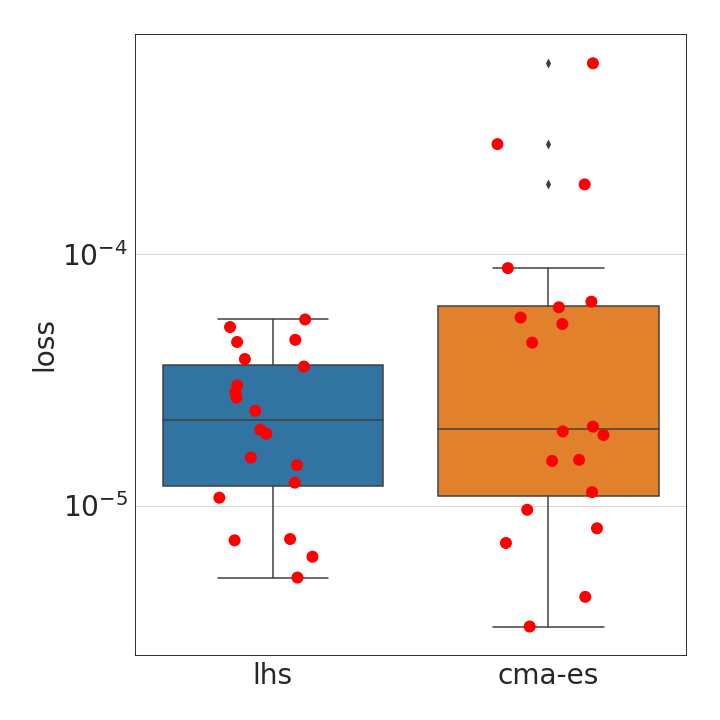
\includegraphics[scale=0.3]{images/lhs_vs_cmaes.png}
\end{figure}

\begin{figure}[h]
\caption{Quality of our approach after the initial sampling vs. initial sampling plus running for further 50 iterations.}
\centering
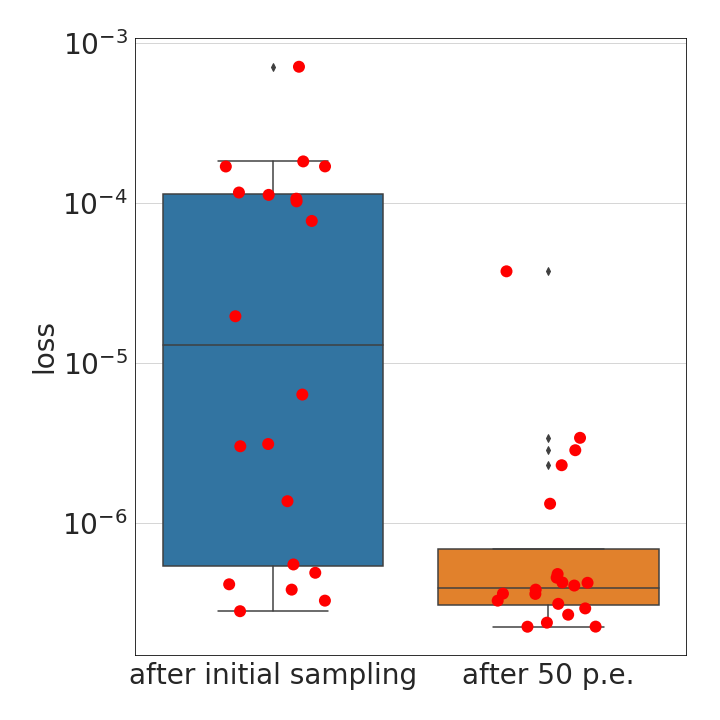
\includegraphics[scale=0.3]{images/two_staged_performancef.png}
\end{figure}


\subsection{Discussion}
%We showed that an initial surrogate model of the objective function build from samples at optimal points of the MM objective function performs better than an initial surrogate model build from samples from a Latin hypercube design in the parameter space.
\section{Conclusion}
New problem of multi-level force field optimization \todo{describe domain again short}, two expensive physics levels, evidence from related work indicates that surrogate-assistance and multilevel optimization works well and we showed that multisurrogate optimization works for this new problem

\paragraph{Future work}
\todo[inline]{AH, multi-*, Wind aus Segeln Optimierungscommunity/reviewers halten}
In-depth comparison of various combinations of surrogate models, optimization, sampling, 

%% The Appendices part is started with the command \appendix;
%% appendix sections are then done as normal sections
%\appendix

%% \section{}
%% \label{}

%% References
%%
%% Following citation commands can be used in the body text:
%% Usage of \cite is as follows:
%%   \cite{key}         ==>>  [#]
%%   \cite[chap. 2]{key} ==>> [#, chap. 2]
%%

%% References with bibTeX database:

\bibliographystyle{elsarticle-num}
\bibliography{Lit.bib}

%% Authors are advised to submit their bibtex database files. They are
%% requested to list a bibtex style file in the manuscript if they do
%% not want to use elsarticle-num.bst.

%% References without bibTeX database:

% \begin{thebibliography}{00}

%% \bibitem must have the following form:
%%   \bibitem{key}...
%%

% \bibitem{}

% \end{thebibliography}


\end{document}

%%
%% End of file 